\documentclass[12pt]{article}
	
%______________________PREAMBULO_________________________

%----------------------Paquetes--------------------------
\usepackage{amsmath,amssymb,amsfonts,latexsym,cancel} % Paquetes de símbolos adicionales.
\usepackage[spanish,es-tabla]{babel} % Idioma español
\usepackage[utf8]{inputenc} % Paquete que nos permite usar los acentos y otros símbolos, directamente del teclado.
\usepackage[T1]{fontenc} % Cambia el tipo de letra
\usepackage{helvet}
\renewcommand*\familydefault{\sfdefault}
%\usepackage{times} % Tipo de letra Times New Roman
\usepackage{graphicx} % Paquete para el manejo de gráficos y figuras en el documento.
\usepackage{geometry} % Permite el manejo de los margenes
\usepackage{fancyhdr} % Permite colocar y manejar el encabezado
\usepackage[breaklinks,colorlinks=true,linkcolor=black,citecolor=blue, urlcolor=blue]{hyperref} % Crea hipervinculo entre secciones y el indice
\renewcommand{\refname}{Bibliografía}
\usepackage{pstricks}
\usepackage{multicol}
\renewcommand{\labelenumi}{$\bullet$}
%\usepackage{mathpazo} %fuente palatino
%\usepackage{xcolor}
%\usepackage[shortlabels]{enumitem}
%-------------Paquetes para el formato de las citas-------
%\usepackage[hyphens]{url}
%\usepackage{float}
%\usepackage{cite}
%\usepackage{wrapfig}

%-----------------------------ayuda de paquetes--------------------

\spanishdecimal{.}

%------------------------Margenes----------------------------

\newgeometry{bottom = 2.5 cm, top = 2.5 cm, left = 3 cm, right = 3 cm} % Modifica el margen {Abajo, Arriba, Izquierda, Derecha

%----------------------------Interlineado----------------------------------

%\doublespacing
%\onehalfspace
%\singlespace
%\spacing{1.5} % Permite personalisar a gusto
%\setlength{\parskip}{2cm} % Es el espacio entre parrafos

%-----------------------------Sangria---------------------------------------

\setlength{\parindent}{0 cm} % Manipula la sangria

%---------------------Portada------------------

%\title{
%\begin{figure}[h!]
		
%	\centering
%	
\includegraphics[width=\linewidth]{Nom_UAdeC_FCFM.png}  			
			
%\end{figure}
%\huge \textbf{LABORATORIO DE FISICA 3}\\\LARGE TITULO PRACTICA\\}
%\author{ \Large \textbf{Profesor:}\\
%\Large \textbf{Alumno:} Oscar Joel Castro Contreras}
%\date{\today}

%--------------Encabezado y pie de pagina--------------------

\pagestyle{fancy}%Coloca el encabezado en el documento
\lhead[]{Física 3}%Encabezado izquierda
\rhead[]{Oscar Joel Castro Contreras}%Encabesado derecha
%\chead[]{}%Encabesado central
\renewcommand{\headrulewidth}{0.08 pt}%Coloca linea al pie de pagina

%\lfoot[]{PI}%Pie de pagina izquerdo
%\rfoot[]{PD}%Pie de pagina derecho
\cfoot[]{\thepage}%Pie de pagina central
\renewcommand{\footrulewidth}{0.08 pt}%Coloca linea al pie de pagina

%-----------------------------------------------------------------------------

	\begin{document}
		
		\begin{titlepage}
		
			\centering
			{\bfseries
			\begin{figure}[h!]
	
				\centering
				
\includegraphics[width=\linewidth]{Nom_UAdeC_FCFM.png}  						
			\end{figure}
			\par}
			\vspace{2cm}
			{\scshape\LARGE FÍSICA 3 \par}
			\vspace{3cm}
			{\scshape\Huge \textbf{El ciclotrón} \par}
			\vfill
			{\LARGE \textbf{Profesor:} Ricardo Pérez Martínez \par}
			\vspace{3cm}
			{\LARGE \textbf{Alumno:} Oscar Joel Castro Contreras \par}
			\vfill
			{\Large \today \par}
			\thispagestyle{empty}
			%\thispagestyle{fancy}
			
		\end{titlepage}
	
		\newpage
		
		\tableofcontents		
		
		\newpage		
		
		\section{¿Que es el ciclotrón?}\label{sec:¿Que es el ciclotrón?}

			\subsection{Historia:}\label{subsec:Historia:}
				El ciclotrón es un tipo de acelerador de partículas que fue desarrollado por los estadounidenses 
				Ernest O. Lawrence (1901-1958) y M. Stanley Livingstone (1905-1986) a principios de la década de 
				1930. \\
				El método directo de acelerar iones utilizando la diferencia de potencial presentaba grandes 
				dificultades experimentales asociados a los campos eléctricos intensos. Existieron iniciativas 
				similares ideadas para acelerar electrones, como los trabajos del físico noruego Rolf Widerøe 
				(1902 - 1996) o las patentes presentadas por el físico húngaro Leo Szilard (1898-1964), pero fueron 
				Lawrence y Livingstone quienes lograron diseñar y construir el ciclotrón que era el primer 
				instrumento de estas características capaz de evita estas dificultades por medio de la aceleración 
				múltiple de los iones hasta alcanzar elevadas velocidades sin el empleo de altos voltajes, 
				transfiriendo a las partículas una energía suficiente como para provocar la desintegración de 
				núcleos atómicos. \\
				Convencido de las aplicaciones de este tipo de máquina. El 26 de enero de 1932, la Oficina de 
				patentes de los Estados Unidos, recibió una solicitud por parte del físico y químico nuclear 
				estadounidense Ernest Orlando Lawrence, para la patente “Método y aparato para acelerar 
				iones”, La patente le fue concedida el 20 de febrero de 1934. \\
				Lawrence promovió la creación de un laboratorio destinado a perfeccionar y mejorar las 
				prestaciones del nuevo instrumento. Fue así como se creó el Radiation Laboratory de la 
				Universidad de California en Berkeley, posteriormente rebautizado en la década de 1970 con el 
				nombre de Lawrence Berkeley Laboratory, en honor a su primer director, una instalación que 
				resultó crucial para el posterior éxito del Proyecto Manhattan.
				\begin{center}
					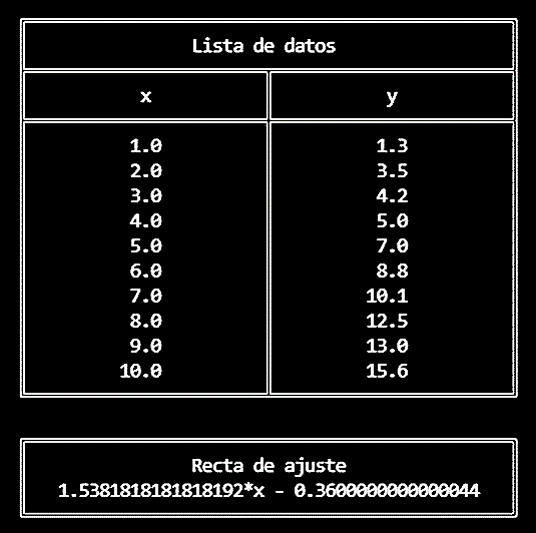
\includegraphics[width=\linewidth]{Figura 1.png}\\
					Figura 1: Imagen de ciclotrón presentada en la patente de Lawrence. \cite{bib:item1}
				\end{center}
				Durante la década de 1930 Lawrence y su equipo se esforzaron por lograr aparatos de un diámetro 
				cada vez mayor con los que conseguir partículas capaces de alcanzar energías cada vez más 
				elevadas: desde su primer ciclotrón de $ 69 cm $ de diámetro, con el que lograron energías de 
				$ 4.8 MeV $, al de $ 152 cm $ de diámetro, que generaba energías de $ 16 MeV $. Su importancia 
				en el desarrollo de la física de partículas fue tal que le valió a Lawrence el Premio Nobel de Física en 
				1939. \\
				La invención que le reportó fama mundial partió de un esbozo en un trozo de papel que se puede ver en la Figura 1. Mientras 
				estaba sentado en la biblioteca una tarde, Lawrence hojeó un artículo y quedó intrigado al ver uno 
				de los diagramas. La idea era producir las partículas de muy alta energía necesarias para la 
				desintegración atómica mediante una sucesión de empujones pequeños. Lawrence les dijo a sus 
				colegas que había encontrado un método para obtener partículas de muy alta energía sin 
				necesitar altos voltajes. \\
				El primer modelo de ciclotrón estaba hecho de alambre y cera. Y funcionó. Cuando Lawrence 
				aplicó $ 2.000 voltios $ de electricidad a su ciclotrón artesanal obtuvo proyectiles de $ 80.000 voltios $. 
				Mediante máquinas cada vez mayores, Lawrence fue capaz de proporcionar el 
				equipamiento necesario para los experimentos de física de altas energías. En 1929 Lawrence 
				diseñó un ciclotrón, capaz de comunicar a las partículas subatómicas una energía de hasta 
				$ 1.200.000 eV $, energía suficiente para provocar la desintegración del núcleo atómico.

			\subsection{En que consiste:}\label{subsec:En que consiste:}
				\begin{center}
					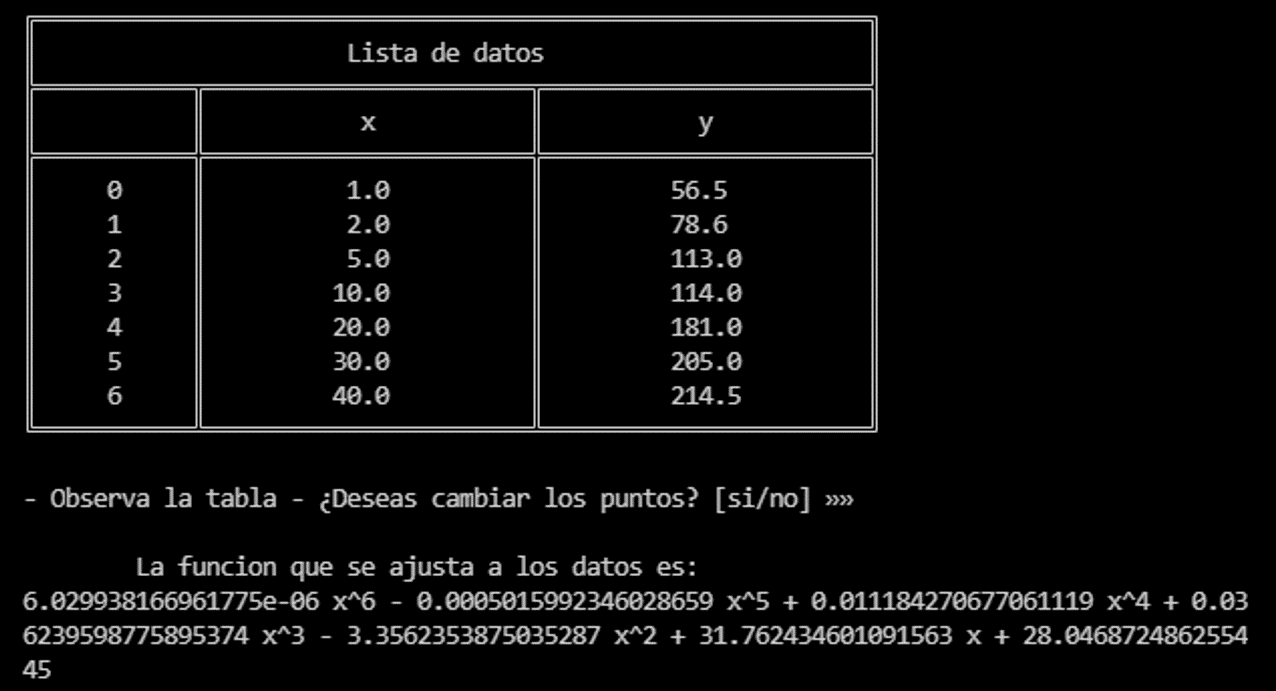
\includegraphics[width=.95\linewidth]{Figura 2.png}\\
					Figura 2: Estructura interna de un ciclotrón. \cite{bib:item2}
				\end{center}
				Un ciclotrón es básicamente una cámara cilíndrica de alto vacío en la que, mediante un campo 
				magnético paralelo al eje del cilindro y un sistema de radiofrecuencia para generar un campo 
				eléctrico alternante, es posible acelerar a energías muy elevadas partículas elementales como 
				protones, producidas mediante una fuente de iones situada en el centro de la cavidad. Estas 
				partículas se hacen chocar con los blancos, en los que tienen lugar reacciones nucleares que 
				llevan a la obtención de los isótopos emisores de positrones. Existen una gran variedad de 
				ellos dependiendo de la potencia, la energía hasta la cual se pueden acelerar las partículas, 
				los blancos a utilizar, etc. \\
				El ciclotrón consta de dos placas semicirculares huecas en forma de ‘D’ llamadas ‘dees’ dentro 
				de una cámara de vacío para que las partículas que viajen por ellas no sean dispersadas en 
				choques con moléculas de los gases que forman el aire. Sobre las "dees" actúa un con un campo 
				magnético uniforme que es perpendicular, generado por un potente electroimán. Las ‘dees’ se montan 
				cara a cara con un espacio estrecho entre ellas, creando un espacio cilíndrico dentro de ellas 
				para que las partículas se muevan. Como se muestra en la figura 2, el punto S es donde se 
				encuentra la fuente que inyecta las partículas, cerca del centro del campo magnético. En las caras 
				se montan 2 placas paralelas, normales al campo magnético en las que se les aplican oscilaciones 
				de alta frecuencia que producen un campo eléctrico oscilante en el espacio que hay entre las ‘dees’ 
				para que la fuerza eléctrica siempre actúe en el sentido del movimiento de las partículas.

			\subsection{Tipos:}\label{subsec:Tipos:}
				\begin{enumerate}
					\item \textbf{Ciclotrón clásico:}
					el primer tipo de ciclotrón, descrito anteriormente que tenía un campo magnético uniforme y una 
					frecuencia constante. Acelerador de partículas en el que se inyecta un chorro de partículas en el 
					seno del campo magnético, que las acelera en una trayectoria circular. A medida que las partículas 
					ganan energía, el campo las obliga a recorrer una espiral creciente, saliendo al final proyectadas 
					en línea recta del acelerador. \\
					\item \textbf{Sincrotrón:}
					es un tipo particular de acelerador de partículas cíclico, que desciende del ciclotrón, en el que el 
					haz de partículas en aceleración viaja alrededor de una trayectoria fija de bucle cerrado. El campo 
					magnético que dobla el haz de partículas en su camino cerrado aumenta con el tiempo durante el 
					proceso de aceleración, sincronizándose con la energía cinética creciente de las partículas. El 
					sincrotrón es uno de los primeros conceptos de acelerador que permite la construcción de 
					instalaciones a gran escala, ya que la flexión, el enfoque del haz y la aceleración se pueden separar 
					en diferentes componentes. Los aceleradores de partículas modernos más potentes utilizan versiones del 
					diseño de sincrotrón. El acelerador de tipo sincrotrón más grande, también el acelerador de partículas 
					más grande del mundo es el Gran Colisionador de Hadrones (LHC) de 27 kilómetros de circunferencia cerca 
					de Ginebra, Suiza, construido en 2008 por la Organización Europea para la Investigación Nuclear (CERN). 
					Puede acelerar haces de protones a una energía de $ 6.5 TeV $. El principio de sincrotrón fue inventado 
					por Vladimir Veksler en 1944. Edwin McMillan construyó el primer sincrotrón de electrones en 1945, y 
					llegó a la idea de forma independiente, habiéndose perdido la publicación de Veksler que solo estaba 
					disponible en una revista soviética. El primer sincrotrón de protones fue diseñado por Sir Marcus Oliphant 
					y construido en 1952.\\
					\item \textbf{Sincrociclotrón:}
					Hay dos diferencias principales entre el sincrociclotrón y el ciclotrón clásico. En el sincrociclotrón, 
					sólo un ‘dees’ conservando su forma clásica, mientras que el otro polo está abierto. Además, la 
					frecuencia del campo eléctrico oscilante en un sincrociclotrón disminuye continuamente en lugar 
					de mantenerse constante para mantener la resonancia del ciclotrón para velocidades relativistas. 
					Un terminal del potencial eléctrico oscilante que varía periódicamente se aplica al ‘dees’ y el otro 
					terminal está en el potencial de tierra. Los protones o deuterones que van a ser acelerados están 
					hechos para moverse en círculos de radio creciente. La aceleración de las partículas se produce 
					cuando entran o salen del ‘dees’. En el borde exterior, el haz de iones se puede quitar con la ayuda 
					de un deflector electrostático. El primer sincrociclotrón produjo deuterones de $ 195 MeV $ y 
					partículas alfa de $ 390 MeV $.\\
					\item \textbf{Microtones:}
					Los microtrones son los ciclotrones más pequeños su función es la aceleración de resonancia de los 
					electrones en el campo eléctrico de frecuencia de microonda. En los imanes de los microtrones se utiliza, 
					generalmente, una inducción del campo magnético pequeña: diez veces menor, aproximadamente, que en los 
					ciclotrones. \\
					\item \textbf{Ciclotrón isócrono o Isociclotrón:}
					una categoría que incluye la mayoría de las máquinas actuales extiende la energía de salida al 
					régimen relativista mediante el uso de piezas polares con forma para crear un campo magnético 
					no uniforme más fuerte en las regiones periféricas para aumentar la fuerza centrípeta sobre la 
					partícula a medida que gana masa relativista para mantener el haz enfocado. Los ciclotrones 
					isócronos permiten elevar la energía de las partículas obtenidas en los aceleradores de ese 
					tipo hasta $ 700-800 MeV $.\\
					\item \textbf{H$^-$Ciclotrón:}
					un ciclotrón que acelera los iones de hidrógeno negativos, lo que facilita la desviación del haz 
					fuera de la máquina. En el punto de salida del haz en la periferia de los ‘dees’, una lámina de metal 
					quita los electrones de los iones de hidrógeno, transformándolos en iones de H$ ^+ $ cargados 
					positivamente. Estos se doblan en la dirección opuesta por el imán, por lo que el rayo abandona la 
					máquina.
				\end{enumerate}

		\section{¿Cuál es la física envuelta en el funcionamiento del ciclotrón?}\label{sec:¿Cuál es la física envuelta en el funcionamiento del ciclotrón?}
			\begin{center}
				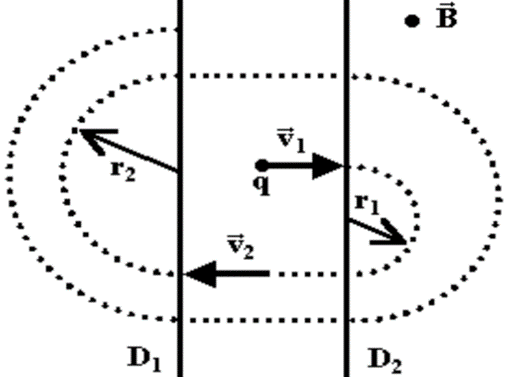
\includegraphics[width=\linewidth]{Figura 3.png}\\
				Figura 2: Movimiento de una particula dentro de un ciclotrón. \cite{bib:item2}
			\end{center}
			El funcionamiento del ciclotrón si nos fijamos en la figura 3, inicialmente se inyecta la partícula 
			cargada $ q $ entrando en la $ D2 $ con una velocidad moderada $ v1 $. Bajo la acción del campo 
			magnético, se ejerce una fuerza magnética la que le proporciona una fuerza que hace que la particula $ q $
			tenga un movimiento circular describiendo una semicircunferencia de radio $ r1 $. Cuando la particula $ q $ 
			sale de la $ D2 $ se le aplica el campo eléctrico generando una fuerza que acelerada la partícula $ q $ 
			entre las dos $ dees $, por la cual entra en la $ D1 $ con una velocidad $ v2 > v1 $. A esa velocidad mayor 
			la particula $ q $ toma un movimiento circular de radio mayor que la primera, describiendo una semicircunferencia 
			de radio $ r2 > r1 $, y vuelven a acceder a la zona entre las ‘dees’, donde se les aplica de nuevo el 
			campo eléctrico, pero ahora en sentido contrario al anterior que vuelve a generar un fuerza que acelerar a 
			la particula $ q $. El proceso se repite una y otra vez hasta que las partículas salen finalmente del ciclotrón 
			a una velocidad muy elevada. Cuando las partículas tienen una velocidad pequeña comparada con el límite superior 
			de velocidades que es la velocidad de la luz, se les puede aplicar las fórmulas de la mecánica de newton, 
			el movimiento circular, la fuerza de un campo eléctrico y la fuerza de Lorentz:\\
			Siguiendo la explicación anterior vemos que la partícula entra en uno de las ‘dees’ donde hay un campo magnético 
			perpendicular, con una velocidad $ v1 $, por lo que podemos usar la fuerza de Lorentz que recordando tiene la 
			formula (1)(2):
			$$ \vec{F} = q(\vec{v} \times \vec{B}) \qquad (1) $$
			$$ F = qvB\sen(\theta) \qquad (2) $$
			Sabiendo que el campo magnético es perpendicular a la velocidad de la particula $ q $, el ángulo $ \theta = 90^0 $ 
			por lo que tendríamos la formula (3):
			$$ F = qvB \qquad (3) $$
			Recordando la segunda ley de Newton en la formula (4):
			$$ F = ma \qquad (4) $$
			Pero como la fuerza esta haciendo que la partícula tenga un movimiento circular, la aceleración centrípeta es la formula (5):
			$$ a = \frac{v^2}{R} \qquad (5) $$
			Por lo que al final la formula de la fuerza que obtenemos dentro de las 'dees' es la formula (6):
			$$ F = qvB = m\frac{v^2}{r} \qquad (6)  $$
			De donde podemos despejar para obtener el radio $ (r) $ y obtenemos la formula (7)
			$$ r = \frac{mv}{qB} \qquad (7)  $$
			Que es la misma fórmula que se aplica en un espectrómetro de masas. Este radio siempre depende de la velocidad, por 
			lo que como la velocidad ira aumentando, el radio de igual forma aumentará con la velocidad.\\
			Pero lo que puede parecer más difícil, es cuando la partícula llega a la parte central donde se genera el campo eléctrico 
			por 2 placas, en esta parte la fuerza que impulsa las partículas seria la de un campo eléctrico por lo que recordando esta 
			dada con la formula (8)
			$$ F = qE \qquad (8) $$
			Y combinando con la segunda ley de newton y recordando que en campo magnético entre 2 placas paralelas esta dado por 
			la formula (9)
			$$ E = \frac{V}{d} \qquad (9) $$
			Llegamos a las fórmulas (10) y (11)
			$$ F = qE = ma \qquad (10) $$
			$$ \frac{qV}{d} = ma \qquad (11) $$
			De aquí podemos ver que la aceleración es lineal, por lo que podemos obtener la aceleración con la que se esta aumentando 
			la velocidad de la partícula, despejándola de la formula (11) y obteniendo la formula (12)
			$$ a = \frac{qV}{dm} \qquad (12) $$
			Vemos que la aceleración de la partícula en esta parte depende de la diferencia de potencial $ (V) $ que se les aplique a las placas y de la 
			distancia $ (d) $ a la que estén separadas. \\
			Pero recordando la explicación el campo eléctrico es oscilatorio, por lo que las placas estarán alternadas entre una carga 
			negativa y un positiva. La carga tiene que estar cambiando cada vez que la partícula pasa por las placas para que esta siga 
			acelerándose, por lo que las placas deben conectarse a una corriente alterna que deber cambiar con una cierta frecuencia, 
			esta frecuencia es con la que la partícula recorre la semicircunferencia que forma en una de las ‘dees’, para obtener esta 
			frecuencia nos ayudaremos de la fórmula del tiempo en el movimiento circular, que es la fórmula (13)
			$$ T = \frac{2\pi r}{v} \qquad (13) $$
			Ahora solo hay que tomar el radio que lo tenemos en la formula (7) y sustituirla en la formula (13), para obtener la formula (14)
			$$ T = \frac{2\pi m}{qB} \qquad (14) $$
			De aquí podemos obtener la frecuencia recodado que la inversa del tiempo como se ve en la formula (15)
			$$ f = \frac{qB}{2\pi m} \qquad (15) $$
			Nosotros tal vez podíamos imaginarnos que este tiempo o la frecuencia en el que alterna el campo eléctrico dependería del radio y la velocidad 
			como en el movimiento circular, pero viendo la formula (14) y (15), todas las variables que tenemos son constantes, por lo que este 
			tiempo en el que alternara el campo eléctrico de las placas también es constante, entonces solo hay que hacer que la fuente 
			alterna a la que conectamos la placas oscilé en este tiempo. A este tiempo se le llama frecuencia ciclotrónica.\\
			Entonces solo nos queda determinar cuanta energía puede generar un ciclotrón, para esto necesitamos la velocidad máxima que 
			puede alcanzar la partícula, esta la podemos obtener de la formula (7) usando el radio máximo que tienen las ‘dees’ y despejando 
			para la velocidad, de esto obtenemos la formula (16)
			$$ v_{max} = \frac{RqB}{m} \qquad (16) $$
			Si vemos con detalle la formula (16), la velocidad máxima de la partícula depende del campo magnético que se ejerza sobre la 
			partícula y del radio que tenga el ciclotrón, por lo que mientras mas grande cea el ciclotrón, con más energía se puede 
			acelerara la partícula. La energía, pues sería energía cinética y usando su fórmula (17)
			$$ k_E = \frac{1}{2}mv^2 \qquad (17) $$
			Donde sustituimos la velocidad máxima de la formula (16) y obtenemos la formula (18).
			$$ k_E = \frac{R^2q^2B^2}{2m} \qquad (18) $$
			O también recordemos que la energía cinética a partir de un campo eléctrico es como se muestra en la formula (19)
			$$ k = qV = \frac{1}{2}mv^2 \qquad (19) $$
			Donde sí analizando desde el inicio por esta parte, podemos ver que al inicio la partícula que se suelta con una velocidad $ (v_1) $ 
			en este punto tendríamos la formula (20)
			$$ qV = \frac{1}{2}mv_1^2 \qquad (20)$$
			Después la partícula regresaría al campo eléctrico gracias al campo magnético y se acelera de nuevo, obteniendo ahora una velocidad 
			$ (v_2) $ entonces, en este punto tenderíamos la formula (21)
			$$ qV + \frac{1}{2}mv_1^2 =  \frac{1}{2}mv_2^2 \qquad (21) $$
			Después de esto de nuevo la partícula regresa al campo eléctrico acelerado y obteniendo ahora una velocidad $ (v_3) $ ahora en este 
			punto tendiéramos la formula (22)
			$$ qV + \frac{1}{2}mv_2^2 =  \frac{1}{2}mv_3^2 \qquad (22) $$
			Si observamos vamos sumando la energía cinética que se le entrega a la partícula en cada vuelta que pasa por el campo eléctrico, 
			por lo que suponemos que la partícula dará $ (N) $ vueltas en el ciclotrón, suponiendo esto llegamos a las formula (23) en la 
			penúltima vuelta y a la formula (24) en la ultima vuelta
			$$ qV + \frac{1}{2}mv_{N-2}^2 =  \frac{1}{2}mv_{n-1}^2 \qquad (23) $$
			$$ qV + \frac{1}{2}mv_{N-1}^2 =  \frac{1}{2}mv_{n}^2 \qquad (24) $$
			Por lo que al final sumando todas estas energías que tomamos en cada vuelta y llegamos a la formula (25)
			$$ 2NqV  =  \frac{1}{2}mv_{n}^2 = \frac{1}{2}mv_{max}^2 \qquad (25) $$

		\section{Problema resuelto por programa de computadora}\label{sec:INTRODUCCIÓN}
			Mi programa yo lo diseñe tratando de que cualquier persona lo entienda, esta muestra un menú con las 
			funcionalidades que tiene desde el cálculo de la energía a la que se puede acelerar la partícula, hasta 
			la velocidad y radio que tiene en cada vuelta que es acelerada la partícula. Lo único que el programa 
			pide es colocar la notación científica de una forma en específico y dar los valores de las variables 
			con una unidad especifica, por ejemplo, la masa la pide en kilogramos, o el radio en metros.\\
			El problema que decidí resolver con mi programa, lo encontré en la referencia \cite{bib:item11}, es un examen de la 
			Olimpiada Española de Física del 8 de marzo 2019.\\
			En un ciclotrón las partículas se mueven en el interior de dos recipientes metálicos semicirculares 
			denominados Ds, los cuales se sitúan dentro de un campo magnético perpendicular proporcionado 
			por un electroimán. En la región en la que se mueven las partículas se realiza vacío para evitar que 
			éstas sean dispersadas al chocar con las moléculas de aire. Entre las Ds se mantiene una diferencia de 
			potencial V que se alterna en el tiempo con un periodo T, igual al periodo de ciclotrón (tiempo que 
			tarda la carga en efectuar una vuelta completa). Esta diferencia de potencial crea un campo eléctrico 
			en el espacio entre las Ds, acelerando las partículas. No existe campo eléctrico dentro de la Ds debido 
			al blindaje metálico.\\
			Considere un ciclotrón de $ 40 cm $ de radio que opera con un campo magnético de $ 0.02 T $ y que acelera protones 
			con una diferencia de potencial de $ 1000 V $. Los protones se emiten en reposo en el punto 1, y a continuación 
			son acelerados por el campo eléctrico antes de entrar en las Ds. Determine:
			\begin{enumerate}
				\item El periodo de ciclotrón $ T $
				\item La velocidad del protón al salir del ciclotrón
			\end{enumerate}

		\section{¿Cuáles son algunas de las aplicaciones del ciclotrón?}\label{sec:¿Cuáles son algunas de las aplicaciones del ciclotrón?}
		
		\section{Conclusión}\label{sec:Conclusión}

		\section{Bibliografía}\label{sec:Bibliografía}
		\renewcommand{\refname}{\vspace{-1cm}}
		\begin{thebibliography}{11}
			\bibitem{bib:item1} Moreira, R. (2005, junio). Principios y elementos de un ciclotrón. Facultades de Medicina e Ingeniería. Univ. de la República Oriental del Uruguay.\\ 
							Recuperado 25 de noviembre de 2021, de \\
							\href{http://www.nib.fmed.edu.uy/Seminario2005/monografias2005/Moreira.pdf}{http://www.nib.fmed.edu.uy/Seminario2005/monografias2005/Moreira.pdf}.
			\bibitem{bib:item2} Castell, P. R. (2020, 25 septiembre). El ciclotrón. Investigación y Ciencia. \\ 
							Recuperado 25 de noviembre de 2021, de \\ 
							\href{https://www.investigacionyciencia.es/blogs/ciencia-y-sociedad/108/posts/el-ciclotrn-18908}{https://www.investigacionyciencia.es/blogs/ciencia-y-sociedad/108/posts/el-ciclotrn-18908}.
		 	\bibitem{bib:item3} Varela, J. (2016, 26 enero). Un instrumento científico para la Historia; el ciclotrón de Lawrence. A hombros de gigantes. Ciencia y tecnología. \\
			 				Recuperado 25 de noviembre de 2021, de \\
							\href{https://ahombrosdegigantescienciaytecnologia.wordpress.com/2016/01/26/un-instrumento-para-la-historia-el-ciclotron-de-lawrwnce/}{https://ahombrosdegigantescienciaytecnologia.wordpress.com/2016/01/26/un-instrumento-para-la-historia-el-ciclotron-de-lawrwnce/}
			\bibitem{bib:item4} tok.wiki. (s. f.). Ciclotrón. hmong. \\
							Recuperado 25 de noviembre de 2021, de \\ 
							\href{https://hmong.es/wiki/Isochronous_cyclotron}{https://hmong.es/wiki/Isochronous\_cyclotron}
			\bibitem{bib:item5} Electromagnetismo. Ciclotrón. (s. f.). TemasElectromagnetismo. \\ 
							Recuperado 25 de noviembre de 2021, de \\ 
							\href{http://rsefalicante.umh.es/TemasElectromagnetismo/Electromagnetismo08.htm}{http://rsefalicante.umh.es/TemasElectromagnetismo/Electromagnetismo08.htm}
			\bibitem{bib:item6} Acelerador de partículas cargadas. El ciclotrón. (s. f.). Acelerador de partículas cargadas. El ciclotrón. \\ 
							Recuperado 25 de noviembre de 2021, de \\ 
							\href{http://www.sc.ehu.es/sbweb/fisica/elecmagnet/ciclotron/ciclo.html}{http://www.sc.ehu.es/sbweb/fisica/elecmagnet/ciclotron/ciclo.html}
			\bibitem{bib:item7} Cyclotron. (s. f.). hyperphysics. \\
			                    Recuperado 25 de noviembre de 2021, de \\ 
							\href{http://hyperphysics.phy-astr.gsu.edu/hbasees/magnetic/cyclot.html}{http://hyperphysics.phy-astr.gsu.edu/hbasees/magnetic/cyclot.html}
			\bibitem{bib:item8} Física 5.02 El Ciclotrón de Ernest Lawrence. (2021, 21 enero). [Vídeo]. YouTube. \\ 
							Recuperado 25 de noviembre de 2021, de \\ 
							\href{https://www.youtube.com/watch?v=l4YUPO0dccU}{https://www.youtube.com/watch?v=l4YUPO0dccU}
			\bibitem{bib:item9} El ciclotrón. (2020, 6 enero). [Vídeo]. YouTube. \\ 
							Recuperado 25 de noviembre de 2021, de \\ 
							\href{https://www.youtube.com/watch?v=QSqZhGXPMq8}{https://www.youtube.com/watch?v=QSqZhGXPMq8}
			\bibitem{bib:item10} 11 04 19 04 CICLOTRON. (2019, 30 abril). [Vídeo]. YouTube. \\
							 Recuperado 25 de noviembre de 2021, de \\  
							 \href{https://www.youtube.com/watch?v=oam9iuNg_dc}{https://www.youtube.com/watch?v=oam9iuNg\_dc}
		\end{thebibliography}
		
	\end{document}